\documentclass{beamer}
\usetheme[progressbar=foot, numbering=counter, block=fill]{metropolis}

\AtBeginSection[]
{
  \begin{frame}<beamer>
    \frametitle{Table of Contents}
    \tableofcontents[currentsection]
  \end{frame}
}

\title{Self regulation of mathematics learning in the college classroom}
\date{April 3, 2018}
\author{Jenny Lee}
\institute{Harvey Mudd College\\Advisor: Dagan Karp}
\begin{document}
\maketitle
\begin{frame}{Recap}
  \begin{itemize}
    \item Mastery based learning and its history
    \begin{itemize}
      \item Problems and challenges
      \item Success in the classroom
    \end{itemize}
    \item Self-paced assessment based learning (SPABL)
    \begin{itemize}
      \item Modifications and adjustments to mastery based learning
    \end{itemize}
    \item Self-paced assessment in the setting of Math 40
  \end{itemize}
\end{frame}
\begin{frame}{The Revised Plan}
  \begin{enumerate}
    \item Narrowing the scope of research
    \item Constructing an annotated bibliography / literature review
    \item Analyzing results of the Math 40 experiment and conducting further follow up research
  \end{enumerate}
\end{frame}
\begin{frame}{Narrowing the scope}
  \begin{center}
    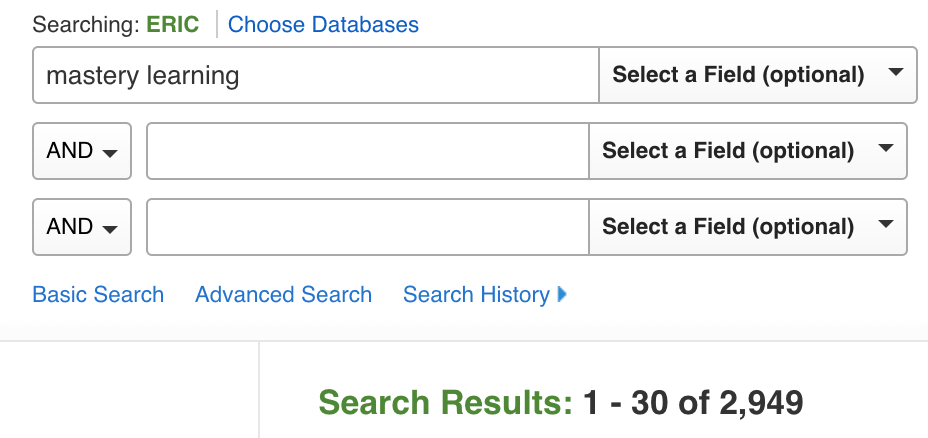
\includegraphics[scale=0.3]{ericsearch}
  \end{center}
  \begin{itemize}
    \item Instruction has evolved and changed in many ways in the last century
    \item Much larger task to examine what has been / what hasn't been studied
    \item Necessary to find a subtopic related to the initial SPABL ideas
  \end{itemize}
\end{frame}
\begin{frame}{Annotated Bibliography - Greg Martin on Gender in Science}
\begin{center}
  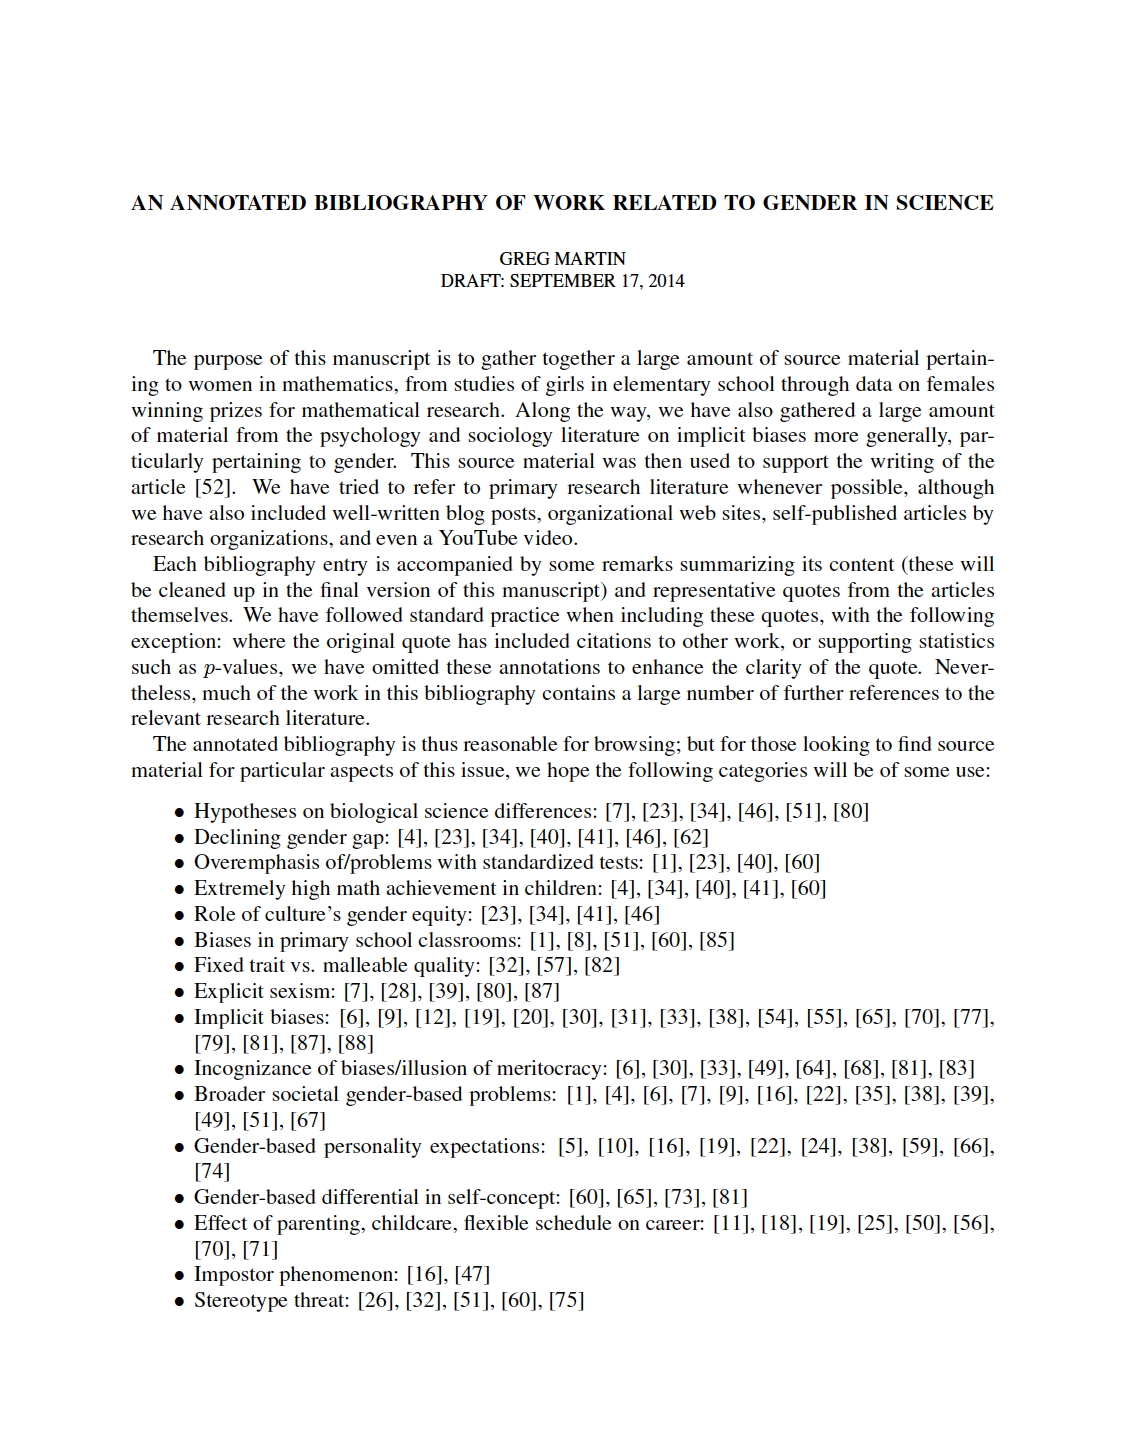
\includegraphics[scale=0.25]{gregmartin2}
  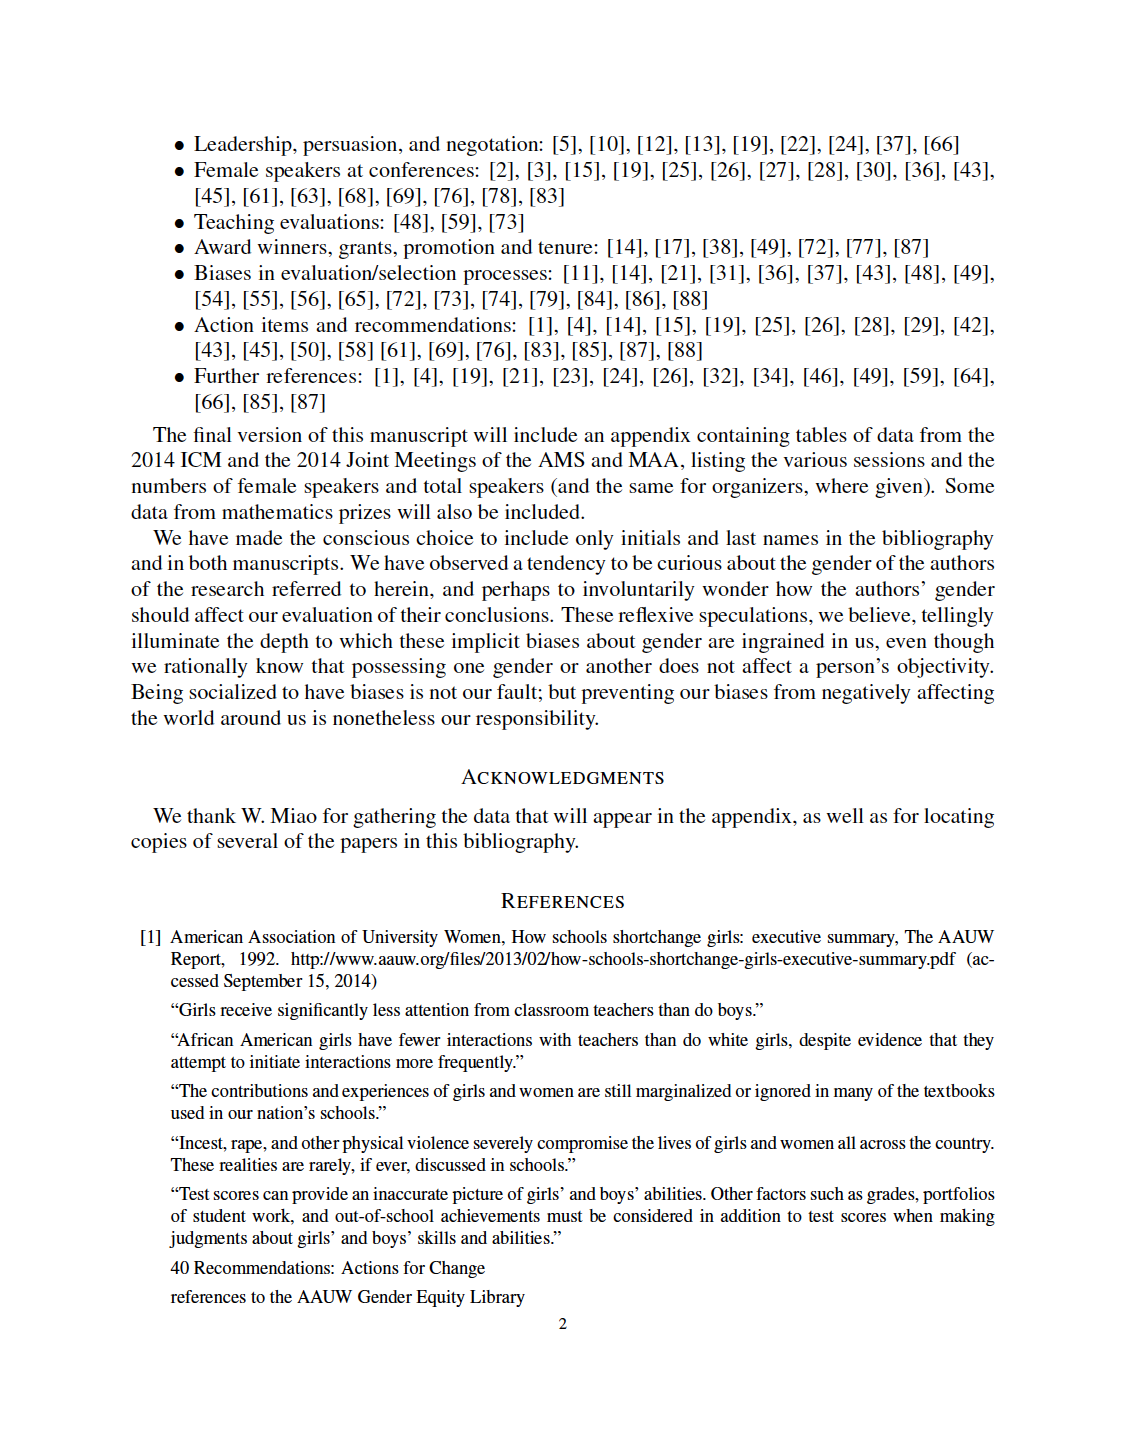
\includegraphics[scale=0.25]{gregmartin3}
\end{center}
\end{frame}
\begin{frame}{Annotated Bibliography - Greg Martin on Gender in Science}
  \begin{itemize}
    \item Categorization of studies and papers written about gender in science
    \item Annotations consist of direct quotes and abstracts, as well as keywords
    \item Goal: Create a reference document easily readable and useful for further studies
  \end{itemize}
\end{frame}
\begin{frame}{Self-regulation and self-paced assessment}
  Definition:
  \begin{center}
    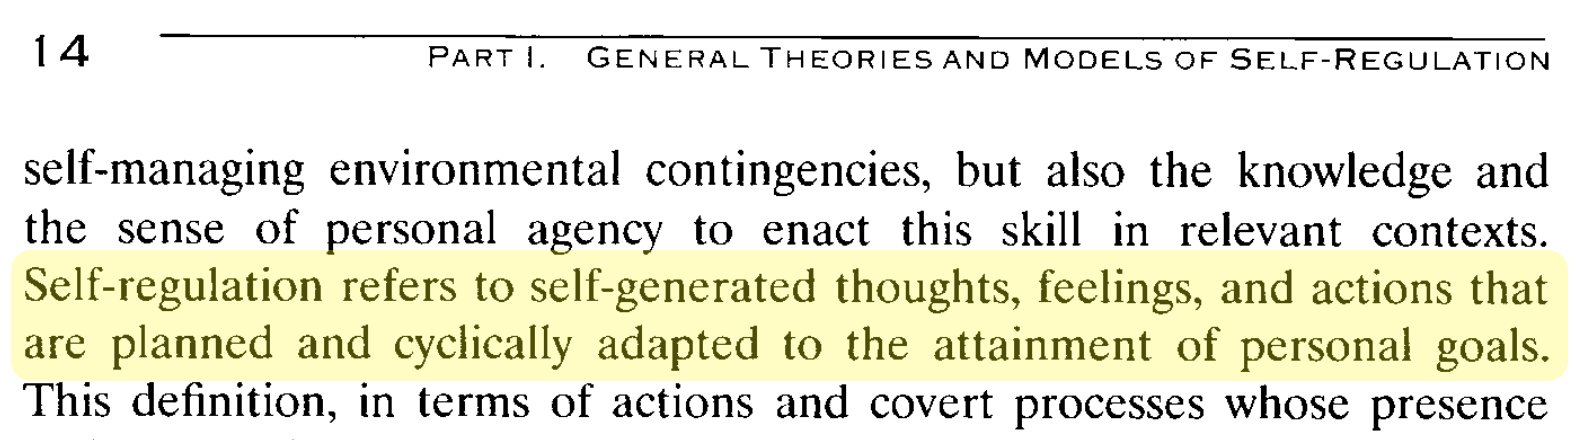
\includegraphics[scale=0.4]{selfregdef}
  \end{center}
  \hfill \begin{minipage}[]{7cm}
      \emph{\tiny Zeidner, M., Pintrich, P. R., \& Boekaerts, M. (2005). Handbook of Self-Regulation. Burlington, MA: Academic Press.}
\end{minipage}

\end{frame}
\begin{frame}{Self-regulation and self-paced assessment}\pause
  \begin{itemize}
    \item Mastery learning has evolved and split into many variations
    \begin{itemize}
      \item IBL (inquiry based learning), flipped classrooms, POGIL (process oriented guided inquiry learning), group learning, online, and many, many more.
    \end{itemize}\pause
    \item Major overlap occurs in fostering independent thought
    \begin{itemize}
      \item Includes developing critical thought (problem solving skills) and forming feelings of self-efficacy (metacognition)
    \end{itemize}
  \end{itemize}
\end{frame}
\begin{frame}{Conducting a meta analysis}\pause
  \begin{itemize}
    \item Restrictions: Mathematics at college/university level institutions
    \begin{itemize}
      \item Empowering minorities and marginalized groups in typically ``neutral'' subject areas
      \item Maturity enables co-creation of knowledge
      \item Specificity calls for tenable solutions
    \end{itemize}\pause
    \item Avoiding studies involving online based classrooms and/or assessments
    \begin{itemize}
      \item Lacks benefits of student-teacher relationships
      \item Feedback is typically standardized and based on purely conceptual understanding
    \end{itemize}\pause
    \item Within last 20 years
  \end{itemize}
\end{frame}
\begin{frame}{Keywords in categorization process}\pause
  \begin{itemize}
    \item Aforementioned, via different learning methods\pause
    \item Outcome (success metrics)
      \begin{itemize}
        \item Quantitative vs. Qualitative
        \item Positive impact vs. No negative impact
      \end{itemize}\pause
    \item Questions raised or answered\pause
    \item ``One variable shy'' from ideal study (stretch)
  \end{itemize}
\end{frame}
\begin{frame}{Extending beyond}\pause
  \begin{itemize}
    \item Is there evidence of consolidation or diversion of the  direction of research?\pause
    \item What influence and/or interaction does this have with other disciplines or settings?\pause
    \item Does it lead to a more equitable practice?
  \end{itemize}
\end{frame}
\begin{frame}{Math 40}\pause
  \begin{itemize}
    \item Currently in post-processing stage of pre- and post-surveys
    \begin{itemize}
      \item Data includes student demographics, prior math knowledge, qualitative feedback, etc.
      \item Thank you, Laura!
    \end{itemize}\pause
    \item Conducting a ``post-post'' survey after completion of Math 65 (ideally summer math for logistical reasons)
    \begin{itemize}
      \item Significance of having ``no negative effect''
    \end{itemize}
  \end{itemize}
\end{frame}
\begin{frame}{Thank you!}
  \centering {\Huge Questions?}
\end{frame}
\end{document}
